% LaTeX file
\documentclass[11pt]{article}
\usepackage{amsmath}
\usepackage{amssymb}
\usepackage{amsthm}
\usepackage{graphicx}
\usepackage{natbib}
\usepackage{tikz}
\usetikzlibrary{calc,patterns,decorations.pathmorphing,decorations.markings}
\usepackage{hyperref}
\title{Lab 7 Analysis}
\author{Abhinav Gupta (120050029) \\ abhinav@cse.iitb.ac.in \\ Anant Gupta (120050086) \\anant@cse.iitb.ac.in\\ Stephan Biastoch (13V051004)\\sbiastoch@cse.iitb.ac.in}
\date{\today}

\begin{document}
\maketitle

\section{Introduction}

This report contains the timing and profiling aspects of the CS296 base code. \\
\\
An iteration count of 10000(unless specified otherwise) has been used for the purpose of profiling.
\\
\\
The code has been timed for the following parameters:
\\1) Different iteration values.
\\2) Different CPU and Memory loads. 
\\
\\
The code has been profiled with the following modes:
\\1) Release Mode: Compilation with level 3 optimization (-O3) and Box2D is built with the Release type.
\\2) Debug Mode: Compilation without any optimization and Box2D is build with the Debug type.
\\
\\
The forthcoming sections analyze the results for each of the cases.
\pagebreak

\section{Timing}
This section explains the interesting phenomena relating to the various time measurements done in lab 5.

\subsection{Average Loop Time}
The average loop time increases with the number of iterations since every iteration takes some fixed amount of time.

\subsection{Average Step Time}
The average step time rapidly decreases at first and then tends to a constant value. This happens since the initialisation of objects takes some finite time, which is distributed over the number of iterations while calculating average step time.

\subsection{Running with heavy processes}
The average loop time and step time increase slightly. However, due to the varying nature of CPU usage the times for different iterations vary unpredictably, and the deviation in step times is also about an order of magnitude higher than normal.
\begin{figure}[h]
\centering
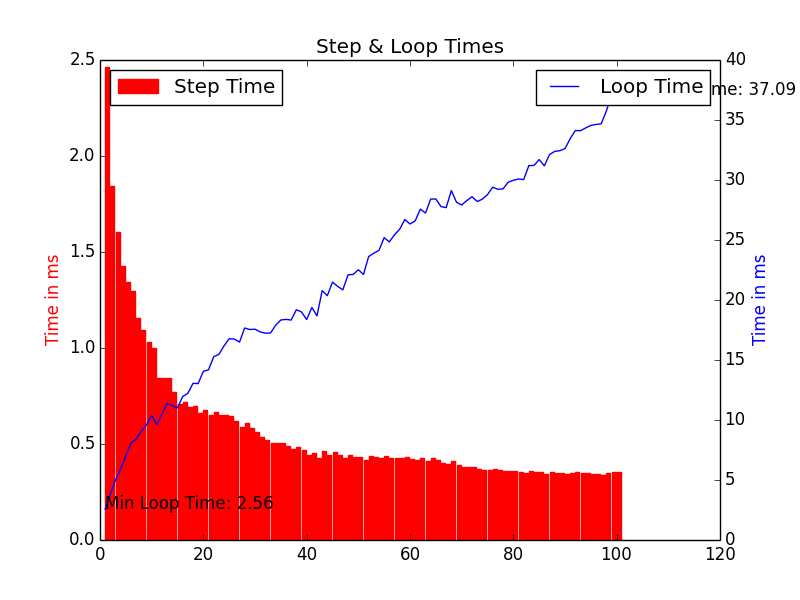
\includegraphics[scale=0.27]{g19_plot01.png}
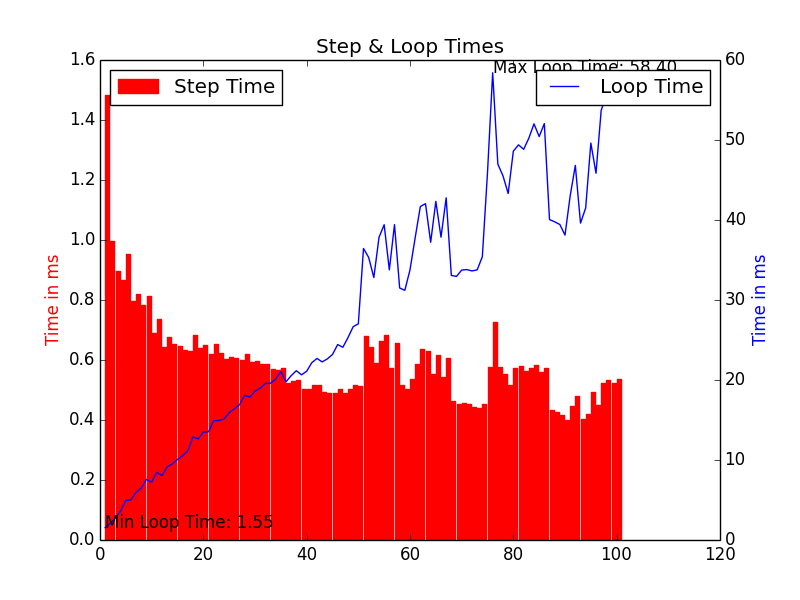
\includegraphics[scale=0.27]{heavy_plot01.png}
\caption{Comparing loop time and step time for normal (left) and heavy (right) CPU usage}
\end{figure}

\begin{figure}[h]
\centering
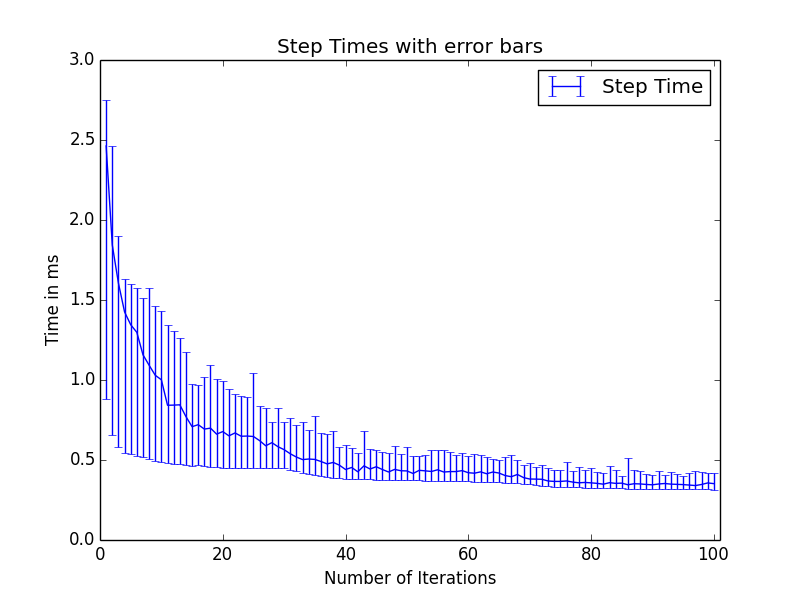
\includegraphics[scale=0.27]{g19_plot03.png}
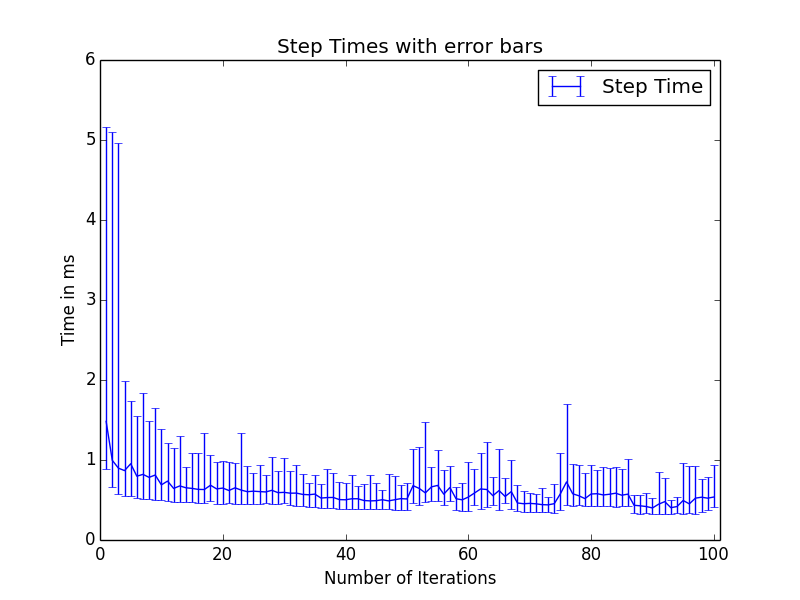
\includegraphics[scale=0.27]{heavy_plot03.png}
\caption{Comparing deviation in step time for normal (left) and heavy (right) CPU usage}
\end{figure}
\subsection{Difference between \textit{time} and \textit{gettimeofday}}
The Unix time command measures the whole program execution time, including the time it takes for the system to load your binary and all its libraries, and the time it takes to clean up everything once your program is finished.

On the other hand, gettimeofday can only work inside your program, that is after it has finished loading (for the initial measurement), and before it is cleaned up (for the final measurement).
\begin{figure}[h]
\centering
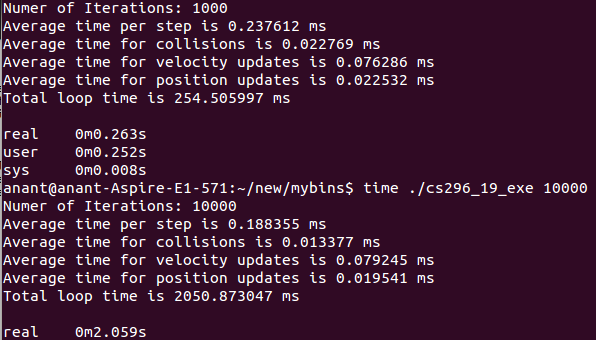
\includegraphics[scale=0.5]{Selection_001.png}
\caption{Difference between output of \textit{time} and loop time (measured using \textit{gettimeofday} is about 9 ms}
\end{figure}

\section{Profiling}
This section analyses the data generated by running GPROF on the executable file, compiled using \textit{release mode} and \textit{debug mode} respectiely.

\subsection{Profile Data}
\textit{Release Mode:}
Since we used level 3 optimization (-O3) while compiling and building the executable and used the Release build type for Box2D, the scope for debugging was suppressed. This was done to achieve a shorter and more efficient code at the expense of the ability to debug.

As a result of the optimization, the code ran for a very short time. (1.5 seconds for 10000 iterations). However few function calls have been listed and analyzed by gprof.
\\
\\
\textit{Debug Mode:}
In this case, the optimization was dropped while compiling and building the executable and the Debug build type was used for Box2D. This resulted in a longer code, albeit with more debugging options.

As a result of this inefficiency, the code ran for a whopping 4 seconds for 10000 iterations. However, the function calls have been elaborately listed and analyzed by gprof.
\\
\subsection{Call Graphs}
\textit{Release Mode:}
Since the function calls have not been fully analysed, the call graph has a very limited structure. Both the number of base functions and the depth of the children function calls is less.
\begin{figure}[h]
\centering
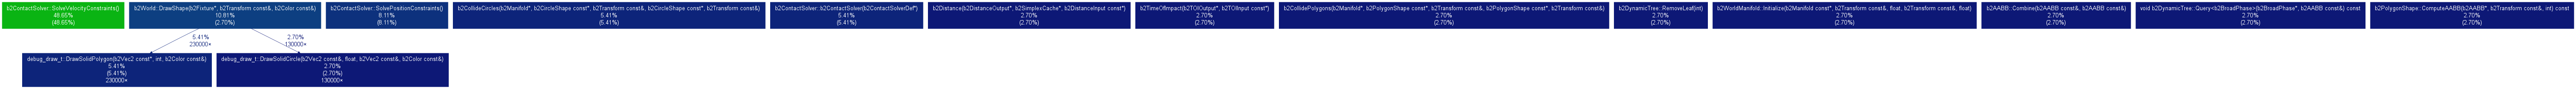
\includegraphics[width=15cm, height=1cm]{out1.png}
\caption{Call graph for the release mode executable generated using \href{https://code.google.com/p/jrfonseca/wiki/Gprof2Dot}{gprof2dot python script}}
\end{figure}
\\
\textit{Debug Mode:}
Since the function calls are properly analysed and listed, the call graph has an extensive structure. There are many root nodes and larger children depth vis a vis the call graph in the release mode.
\begin{figure}[h]
\centering

\includegraphics[width=15cm, height=1cm]{out2.png}
\caption{Call graph for the debug mode executable generated using \href{https://code.google.com/p/jrfonseca/wiki/Gprof2Dot}{gprof2dot python script}}
\end{figure}
\\
\subsection{Function to be optimized}
The SolveVelocityConstraints function has taken up a lot of processing time as is evident in both the Release and Debug Modes. It's share is much larger in the Release Mode which is more important as that is the actual version to be used. Hence this function can potentially be optimized.
\begin{figure}[h]
\centering
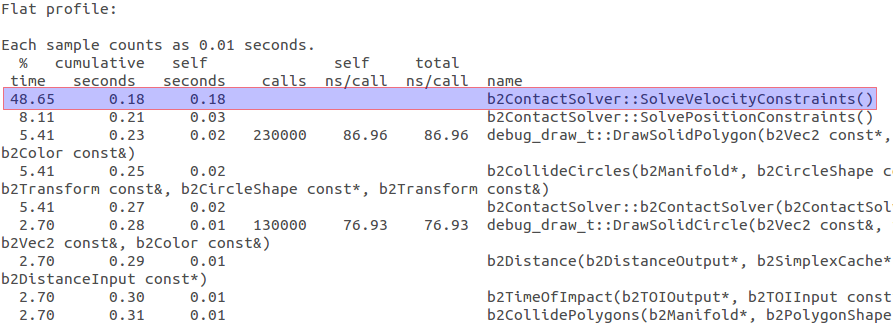
\includegraphics[scale=0.4]{Selection_002.png}
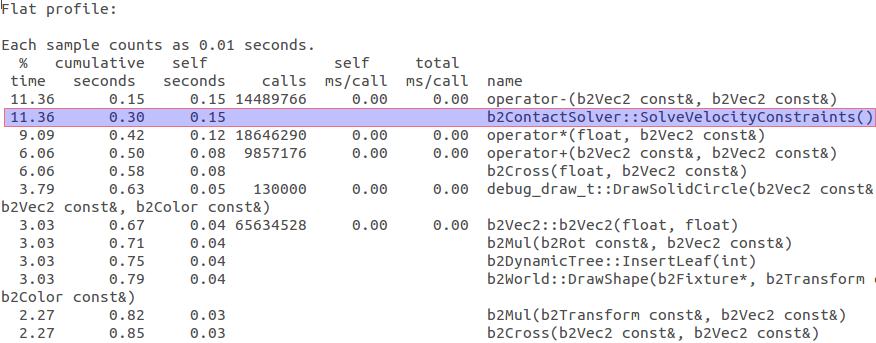
\includegraphics[scale=0.4]{Selection_003.png}
\caption{Clearly, the \textit{solveForVelocity} function is the bottleneck in both \textit{release} (top) and \textit{debug} (bottom) modes}
\end{figure}

\bibliographystyle{te}
\end{document}
